\newpage
\section{Wasserkraftwerk-Typen}

\subsection{Klassifizierung}

\begin{itemize}
    \item Laufwasserkraftwerke
    \item Mitteldruckanlagen
    \item Hochdruck- (Speicher-) Anlagen
    \item Pumpspeicherkraftwerke
    \item Gezeitenkraftwerke
    \item Wellenkraftwerke
    \item Wasserwirbelkraftwerke
\end{itemize}


\subsection{Einteilung nach technischen Aspekten}
\begin{itemize}
    \item \textbf{Laufwasserkraftwerke}
    \begin{itemize}
        \item Flusskraftwerke
        \begin{itemize}
            \item Blockbauweise
            \item Buchtenkraftwerke
            \item Zwillingsbauweise (beidseitige Anordnung)
            \item \dots
        \end{itemize}
        \item Ausleitungskraftwerke
    \end{itemize}
    
    \item \textbf{Speicherkraftwerke} mit natürlichem Zufluss
    \item \textbf{Pumpspeicherkraftwerke} (Speicherkraftwerke mit oder ohne natürlichem Zufluss)
    \item Gezeitenkraftwerke
    \item Wellenkraftwerke
\end{itemize}



\subsection{Einteilung nach energiewirtschaftlichen Aspekten}
\begin{itemize}
    \item Grundlastkraftwerke (häufig verwendet, Laufwasser, Speicher mit vielen Volllaststunden)
    \item Mittellastkraftwerke
    \item Spitzenlastkraftwerke (Speicher mit wenig Volllaststunden)
\end{itemize}



\subsection{Einteilung nach Betriebsart}
\begin{itemize}
    \item Verbundbetrieb (im Normalbetrieb alle Kraftwerke in der Schweiz)
    \item Inselbetrieb (Unabhängig vom Netz)
\end{itemize}



\subsection{Einteilung nach der installierten Leistung}
\begin{itemize}
    \item Kleinwasserkraftwerke (in der Regel kleiner 10 MW)
    \item Grosswasserkraftwerke (P > 10 MW)
\end{itemize}



\subsection{Einteilung nach wasserwirtschaftlichen Aspekten}
\begin{itemize}
    \item Wasserkraftwerke, die ausschliesslich elektrische Energie produzieren
    \item Wasserkraftanlagen für mehrere wasserwirtschaftliche Zielsetzungen (Mehrzweckanlagen, z.\,B. Trinkwasser)
\end{itemize}



\subsection{Wasserturbinen und Pumpen}

\begin{itemize}
    \item \textbf{Aktionsturbinen:} Arbeit aus kinetischer Energie-Differenz
    \begin{itemize}
        \item \textbf{Peltonturbinen}
    \end{itemize}

\item \textbf{Reaktionsturbinen:} Arbeit aus Druckdifferenz vor und nach Turbine
    \begin{itemize}
        \item Francisturbinen (spiralförmig)
        \item Kaplanturbinen (propellerförmig)
        \item Rohrturbinen
        \item Kreiselpumpen als Turbinen
    \end{itemize}
\end{itemize}



\subsection{Laufwasserkraftwerke LWK}

\begin{center}
    \includegraphics[width=0.95\columnwidth, align=c]{images/Laufwasserkraftwerke.png}
\end{center}

\begin{minipage}[c]{0.38\columnwidth}
    \begin{tabular}{c l}
        1 & Oberwasser \\ 
        2 & Unterwasser \\ 
        3 & Maschinenhaus \\
        4 & Stauwehr \\
        5 & Transformatoren \\
    \end{tabular}
\end{minipage}
\hfill
\begin{minipage}[c]{0.58\columnwidth}
    \begin{tabular}{c l}
        6 & Schaltanlage \\
        7 & Leitungen \\
        8 & Betriebsgebäude \\
        9 & Fischtreppe \\
        10 & Einrichtung für den Schiffstransport \\
    \end{tabular}
\end{minipage}



\subsection{LWK mit Kaplanturbinen Vertikal}

\begin{center}
    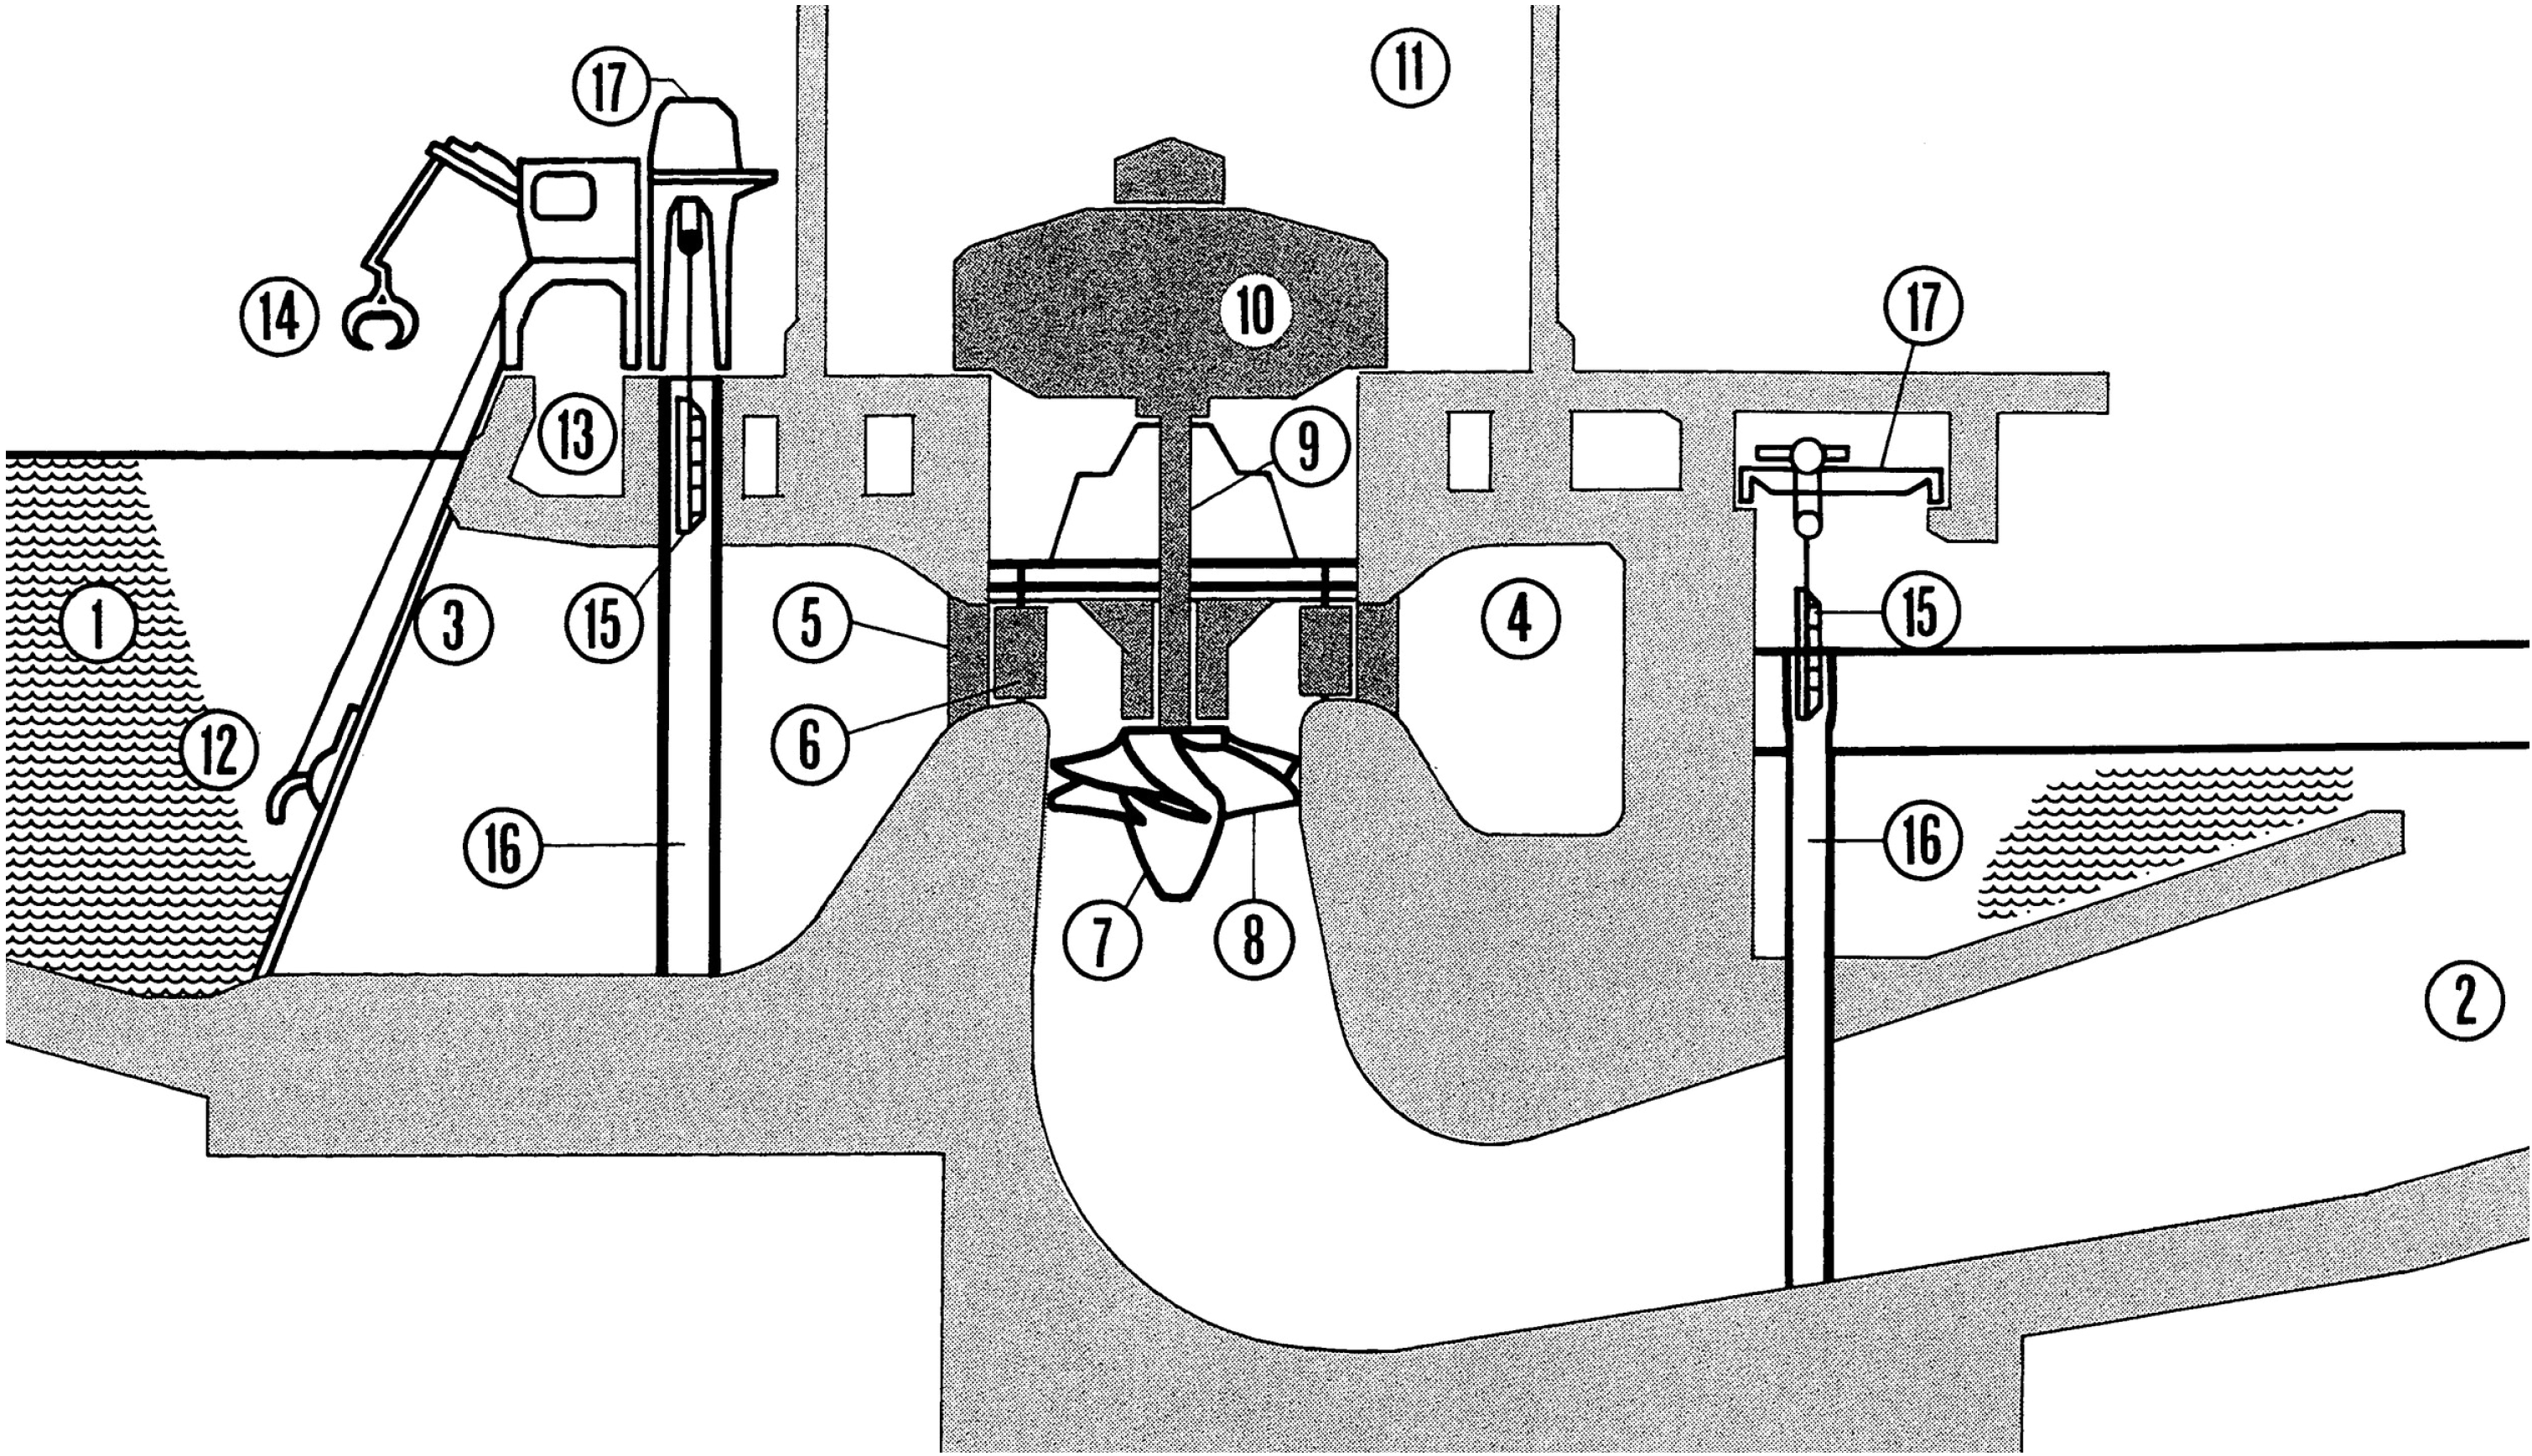
\includegraphics[width=0.95\columnwidth, align=c]{images/Laufwasserkraftwerke_Kaplanturbine_Vertikal.png}
\end{center}

\begin{minipage}[t]{0.38\columnwidth}
    \begin{tabular}{c l}
        1 & Oberwasser \\
        2 & Unterwasser \\
        3 & Rechen \\
        4 & Spirale \\
        5 & Stützschaufeln \\
        6 & Leitschaufeln \\
        7 & Laufrad \\
        8 & Laufradschaufeln \\
        9 & Saugrohr \\
    \end{tabular}
\end{minipage}
\hfill
\begin{minipage}[t]{0.58\columnwidth}
    \begin{tabular}{c l}
        10 & Generator \\
        11 & Maschinenhaus \\
        12 & Rechenreinigungsmaschine \\
        13 & Geschwemmselrinne \\
        14 & Zangengreifer \\
        15 & Dammbalken \\
        16 & Nuten für Dammbalken \\
        17 & Dammbalkenkran \\
           &  \\
    \end{tabular}
\end{minipage}



\subsection{LWK mit Kaplanturbinen Horizontal}

\begin{center}
    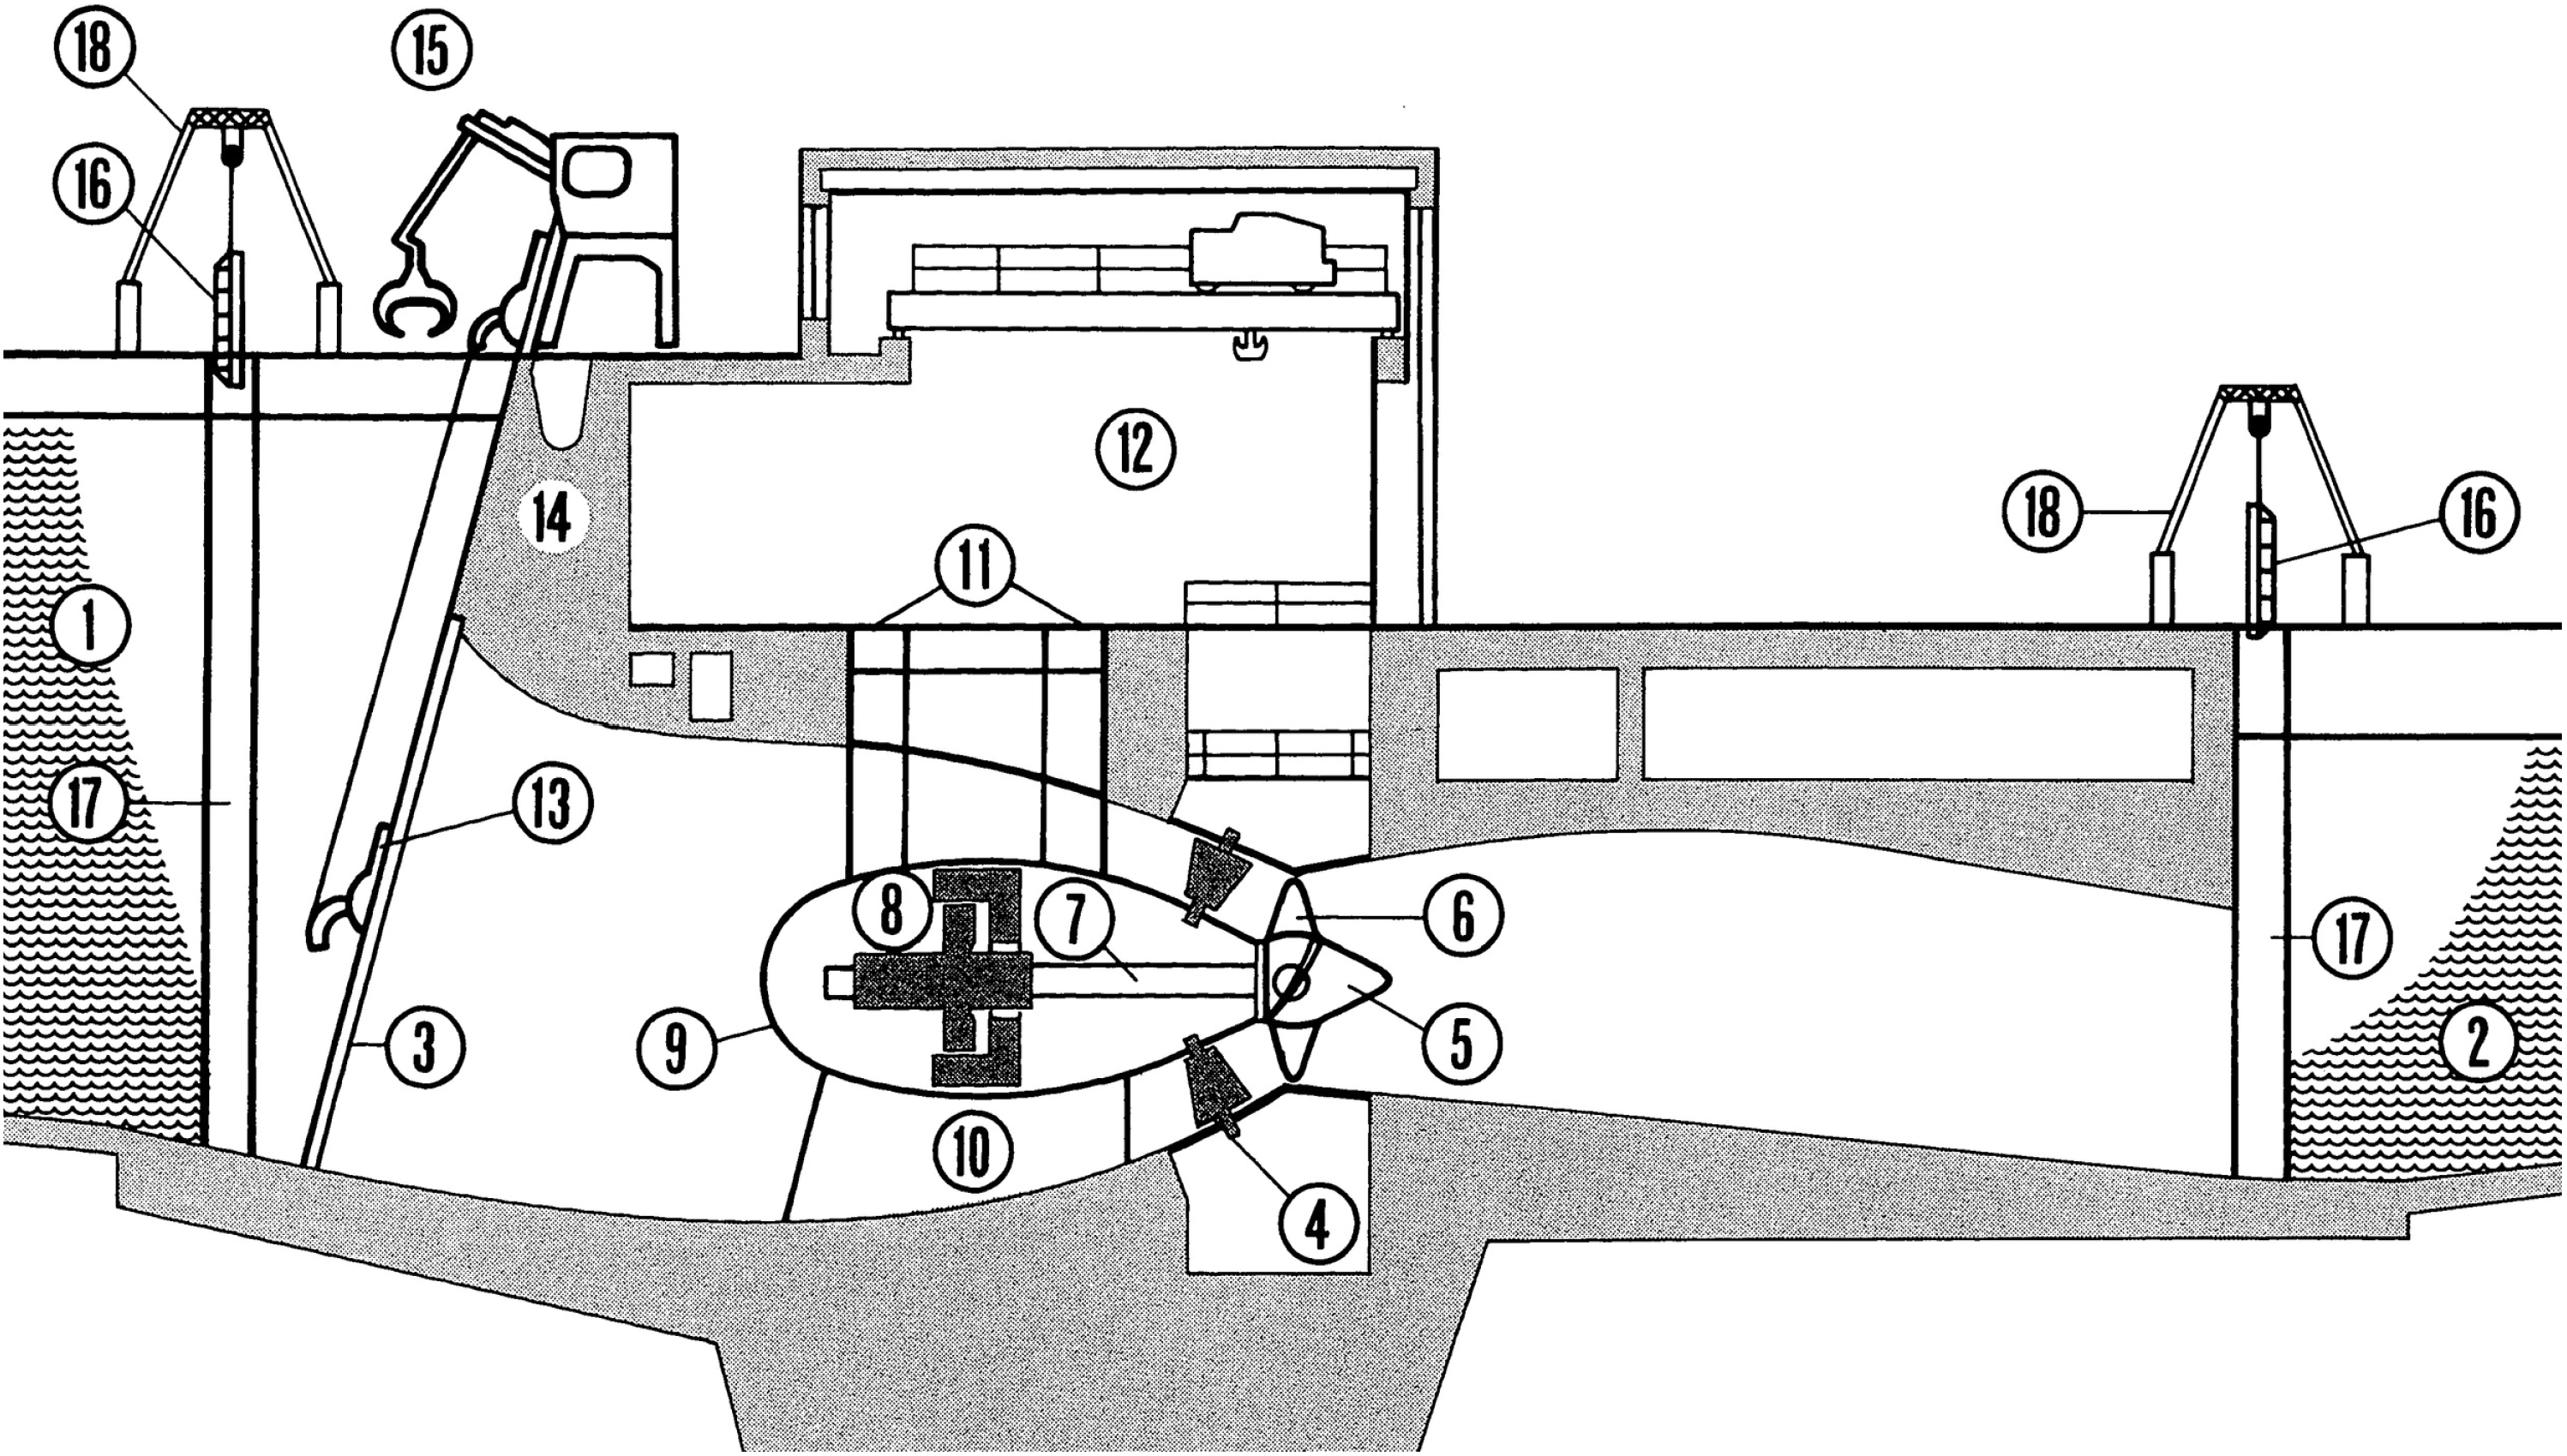
\includegraphics[width=0.95\columnwidth, align=c]{images/Laufwasserkraftwerke_Kaplanturbine_Horizontal.png}
\end{center}

\begin{minipage}[t]{0.38\columnwidth}
    \begin{tabular}{c l}
        1 & Oberwasser \\
        2 & Unterwasser \\
        3 & Rechen \\
        4 & Leitschaufeln \\
        5 & Laufrad \\
        6 & Laufradschaufeln \\
        7 & Turbinenwelle \\
        8 & Generator \\
        9 & Gehäuse \\
    \end{tabular}
\end{minipage}
\hfill
\begin{minipage}[t]{0.58\columnwidth}
    \begin{tabular}{c l}
        10 & Sockel \\
        11 & Einstiegsschächte \\
        12 & Maschinenhalle \\
        13 & Rechenreinigungsmaschine \\
        14 & Geschwemmselrinne \\
        15 & Zangengreifer \\
        16 & Dammbalken \\
        17 & Nuten für die Dammbalken \\
        18 & Dammbalkenkran \\
    \end{tabular}
\end{minipage}




































